\documentclass[a4paper,12pt]{report}
\usepackage[toc,page]{appendix}
\usepackage{amsmath}
\usepackage{float}
\usepackage{graphicx}
\usepackage{subfig}
\usepackage{amssymb}
\usepackage{geometry}
\usepackage{array}
\usepackage{tcolorbox}
\usepackage[normalem]{ulem}

\usepackage{setspace}
 \geometry{
 a4paper,
 total={170mm,257mm},
 left=20mm,
 top=20mm,
 }
\usepackage{tikz}
\usepackage{pgfplots}
\usetikzlibrary{shapes, arrows.meta, decorations.pathreplacing, positioning, petri, fit, calc}
\tikzstyle{startstop} = [circle, minimum size=1cm ,text centered, draw=black]
\tikzstyle{neuron} = [circle, minimum size=1cm ,text centered, draw=red, fill=gray!30]
\tikzstyle{neuronEll} = [ellipse, minimum size=1cm ,text centered, text width=2cm, draw=red, fill=gray!30]
\tikzstyle{process} = [rectangle, minimum width=2cm, minimum height=0.5cm, text centered, text width=3cm, draw=black, fill=blue!30]
\tikzstyle{detail} = [rectangle, minimum width=1.5cm, minimum height=0.5cm, text justified, text width=2.6cm, fill=white!30]
\tikzstyle{smalldetail} = [rectangle, minimum width=2cm, minimum height=1cm, text centered, text width=2cm]
\tikzstyle{largedetail} = [rectangle, minimum width=3cm, minimum height=1cm, text centered, text width=4cm, fill=white!30]
\tikzstyle{box} = [rectangle, minimum width=5cm, minimum height=9cm, text centered, text width=4cm, draw=black, fill=white!30]

\usepackage[utf8]{inputenc}

% Default fixed font does not support bold face
\DeclareFixedFont{\ttb}{T1}{txtt}{bx}{n}{10} % for bold
\DeclareFixedFont{\ttm}{T1}{txtt}{m}{n}{10}  % for normal

% Custom colors
\usepackage{color}
\definecolor{deepblue}{rgb}{0,0,0.5}
\definecolor{deepred}{rgb}{0.6,0,0}
\definecolor{deepgreen}{rgb}{0,0.5,0}

\usepackage{listings}
\usepackage{mathtools}
% Python style for highlighting
\newcommand\pythonstyle{\lstset{
language=Python,
basicstyle=\ttm,
otherkeywords={self},             % Add keywords here
keywordstyle=\ttb\color{deepblue},
emph={MyClass,__init__},          % Custom highlighting
emphstyle=\ttb\color{deepred},    % Custom highlighting style
stringstyle=\color{deepgreen},
frame=tb,                         % Any extra options here
showstringspaces=false            % 
}}


% Python environment
\lstnewenvironment{python}[1][]
{
\pythonstyle
\lstset{#1}
}
{}

% Python for external files
\newcommand\pythonexternal[2][]{{
\pythonstyle
\lstinputlisting[#1]{#2}}}

% Python for inline
\newcommand\pythoninline[1]{{\pythonstyle\lstinline!#1!}}


\begin{document}
\tableofcontents

\title{Anomaly Detection (Unsupervised) \\ and  \\ Recommender Systems}
\maketitle
\part{Week 9}
\section{Anomaly Detection: Intuition}
Given a dataset $\{ x^{(1)}, x^{(2)}, ..., x^{(m)}  \}$, the goal is to determine whether a new example $x^{\text{test}}$ is anomalous. \\
We model $p(x)$ and then evaluate $p(x^{\text{(test)}})$: $\begin{dcases}  \text{if\ } p(x^{\text{(test)}}) \leq \epsilon & \rightarrow \text{flag anomaly} \\
\text{if\ } p(x^{\text{(test)}}) > \epsilon & \rightarrow \text{OK} \end{dcases}$
\section{Review of Gaussian Distribution}
If $x (\in \mathbb{R})$ is a distributed Gaussian with mean $\mu$, variance $\sigma^2$: i.e $x \sim \aleph(\mu, \sigma^2)$, where '$\sim$' stands for 'distributed as'. The propability of $x$ parametrized by $\mu$ and $\sigma^2$ ($x \sim \aleph(\mu, \sigma^2)$) is :
\begin{align}
p(x; \mu, \sigma^2) = \frac{1}{\sqrt{2 \pi} \sigma} \text{exp}\left[-\frac{(x-\mu)^2}{2 \sigma^2} \right]
\end{align}
\begin{figure}[H]
\centering
        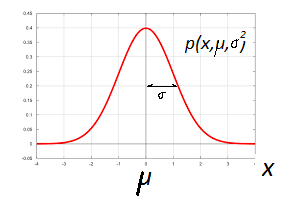
\includegraphics[totalheight=4 cm]{gaussian.png}
\end{figure}

\subsection{Parameter estimation}
Given a dataset $\{x^{(1)}, x^{(2)}, ..., x^{(m)}  \}$, where $x^{(i)} \in \mathbb{R}$, for which we suspect each example come from a Gaussian distribution ($x^{(i)} \sim \aleph(\mu, \sigma^2)$:
\begin{align}
\begin{split}
\mu &= \frac{1}{m} \sum_{i=1} ^m x^{(i)} \\
\sigma^2 &= \frac{1}{m} \sum_{i=1} ^m (x^{(i)}-\mu)^2
\end{split}
\end{align}

\section{Anomaly detection}
\subsection{Density estimation: $p(x)$}
Given a training set  $\{ x^{(1)}, x^{(2)}, ..., x^{(m)}  \}$, where $x^{(i)} \in \mathbb{R}^n$. We model $p(x)$ from the dataset :
\begin{align}
p(x) = \prod _{j=1} ^n p(x_j; \mu_j, \sigma_j ^2) = p(x_1; \mu_1, \sigma_1 ^2) p(x_2; \mu_2, \sigma_2 ^2) p(x_3; \mu_3, \sigma_3 ^2) ....p(x_n; \mu_n, \sigma_n ^2) 
\end{align}
We assume that the probability of first feature, $p(x_1)$, 2nd feature $p(x_2),...$ are Gaussian probability distributions, i.e : $x_1 \sim \aleph(\mu_1, \sigma_1 ^2)$, $x_2 \sim \aleph(\mu_2, \sigma_2 ^2)$, etc...$x_n \sim \aleph(\mu_n, \sigma_n ^2)$
\begin{itemize}
\item The formulation of $p(x)$ assumes that the features are independent (not corrolated), but in fact the algorithm works for both (independent and not).
\end{itemize}

\subsection{Anomaly Detection Algorithm}
\begin{enumerate}
\item Given an unlabeled training set $\{x^{(1)}, x^{(2)}, ..., x^{(m)}  \}$
\item Fit parameters $\mu_1, \mu_2, ..., \mu_n, \sigma_1 ^2, \sigma_2 ^2,..., \sigma_n ^2$, which can be written in a vectorized form:
\begin{align}
\begin{split}
\mu = \left[ \begin{smallmatrix} \mu_1 \\ \mu_2 \\ ..\\..\\..\\ \mu_n \end{smallmatrix} \right] & ,\text{where: \ }  \mu_j= \frac{1}{m} \sum _{i=1} ^m x_j ^{(i)} \\
\sigma ^2 = \left[ \begin{smallmatrix} \sigma_1 ^2 \\ \sigma_2 ^2 \\ ..\\..\\..\\ \sigma_n ^2 \end{smallmatrix} \right] & , \text{where: \ } \sigma_j ^2 = \frac{1}{m} \sum _{i=1} ^m (x_j ^{(i)} - \mu_j ^{(i)})^2
\end{split}
\end{align}
\item Given new example $x$, compute $p(x)$:
\begin{align}
p(x) = \prod_{j=1} ^n p(x_j; \mu_j, \sigma_j ^2) = \prod_{j=1} ^n \frac{1}{\sqrt{2 \pi} \sigma_j} \text{exp} \left[ -\frac{(x_j-\mu_j)^2}{2 \sigma_j ^2} \right]
\end{align}
If $p(x) < \epsilon $ then $x$ is tagged as an anomaly
\end{enumerate}

\subsection{Evaluate an anomaly detection system}
Example of aircraft engines: we have a dataset with 10,000 good/normal engines ($y=0$) and 20 flawed engines/anomalous ($y=1$)
\begin{enumerate}
\item Training set: 6,000 good engines ($y=0$) \\
Fit model $p(x)$ on training set $\{x^{(1)}, x^{(2)}, ..., x^{(m)}  \}$
\item Cross validation set: 2,000 good engines of dataset with both $y=0$ and $y=1$
\item Test set: 2,000 good engines of dataset with both $y=0$ and $y=1$
\begin{itemize}
 \item On CV and Test examples, predict $x^{(test)}, y^{(test)}$
\item Use CV to choose parameter $\epsilon$
\item if $p(x)$ is about same when $y=0$ and $y=1$, use a new feature.
\end{itemize}
\end{enumerate}

\begin{itemize}
\item Possible evaluation metrics:
\begin{itemize}
\item True Positive/False Positive, True Negative/False Negative
\item Precision/Recall
\item F1-score
\end{itemize}
\end{itemize}
*Because the dataset is typically skewed (much less $y=1$ count than $y=0$), predicting $y=0$ would have a very high accuracy.

\subsection{Anomaly detection vs. supervised Learning}
\begin{table}[H]
\begin{tabular}{|  >{\centering\arraybackslash} m{8cm} | >{\centering\arraybackslash} m{8cm}  |}
\hline
\textbf{Anomaly Detection} & \textbf{Supervised Learning} \\[2ex]
\hline
Very small number of positive examples ($y=1$): 10-50, and Large Number of Negative examples & Large Number of positive and Negative examples \\
\hline
Many different types of anomalies (hard for algorithm to learn from positive examples, what the anomalies look like; future anomalies may look different that the anomalous examples seen so far) & Enough positive examples for the algorithm to get a sense of what positive example is : future positive examples likely to be similar to ones in training set \\
\hline
Application: Fraud Detection, Manufacturing (aircraft engines, etc...), Monitoring Machines in a data center... & email spam classification, weather prediction (sunny/rainy, etc...), cancer classification \\
\hline
\end{tabular}
\end{table}
\subsection{Features selection}
\begin{itemize}
\item It is important to check whether the data is Gaussian.
\item if the data is not Gaussian, transform it to make it look Gaussian. Some examples of feature Transformation:
\begin{align}
\begin{split}
x_2 \leftarrow log(x_2) \\
x_2 \leftarrow log(x_2 + c) \\
x_2 \leftarrow \sqrt{x_2} \\
x_2 \leftarrow x_2 ^{1/3}
\end{split}
\end{align}
\end{itemize}
\section{Multivariate Gaussian (Normal) distribution}
\section{Density Estimation}
Instead of modeling $p_x = p(x_1)p(x_2)...p(x_n)$ where $p(x_j)$ are calculated separately, Multivariate Gaussian models $p(x)$ all in one-go, using the parameters $\mu \in \mathbb{R}^n$ and $\Sigma \in \mathbb{R}^{n \times n}$ (covariance matrix): 
\begin{align}
p(x; \mu, \Sigma) = \frac{1}{(2 \pi)^{n/2} |\Sigma|^{1/2}} \text{exp} \left[-\frac{1}{2}(x-\mu)^T \Sigma ^{-1} (x - \mu) \right] 
\end{align}
where $|\Sigma|$ is the determinant of the covariance matrix. \\
* Octave uses det(Sigma) for determinant of Sigma
\subsection{Algorithm}
\begin{enumerate}
\item Given a training set $\{x^{(1)}, x^{(2)}, ..., x^{(m)}  \}$ where $x \in \mathbb{R}^n$ comes from a multivariate Gaussian distribution.
\item Model: 
\begin{align}
p(x; \mu, \Sigma) = \frac{1}{(2 \pi)^{n/2} |\Sigma|^{1/2}} \text{exp} \left[ -\frac{1}{2}(x-\mu)^T \Sigma ^{-1} (x - \mu) \right]
\end{align}
where
\begin{align}
\begin{split}
\mu &= \left[ \begin{smallmatrix} \mu_1\\ \mu_2 \\..\\..\\ \mu_n \end{smallmatrix} \right] = \frac{1}{m} \sum_{i=1} ^m x^{(i)} \\
\Sigma &= \frac{1}{m} \sum_{i=1} ^{m} (x^{(i)} - \mu)(x^{(i)} - \mu)^T
\end{split}
\end{align}
\item Given a new example $x$, compute :
\begin{align}
p(x; \mu, \Sigma) = \frac{1}{(2 \pi)^{n/2} |\Sigma|^{1/2}} \text{exp} \left[-\frac{1}{2}(x-\mu)^T \Sigma ^{-1} (x - \mu) \right] 
\end{align}
\begin{itemize}
 \item if $p(x) < \epsilon $, $x$ is an anomaly
\end{itemize}
\end{enumerate}

\subsection{Original Model versus Multi-Variate}
\begin{itemize}
\item The original model corresponds to the multivariate model when the off-diaginal elements of $\Sigma$ are zero, i.e:
\begin{align}
\Sigma = \left[ \begin{smallmatrix} \sigma_1 ^2 &0&0..&0 \\ 0&\sigma_2^2&0..&0 \\ 0&0&....&0 \\0&0&....&0 \\ 0&0&0..&\sigma_n^2 \end{smallmatrix} \right]
\end{align}

\end{itemize}

\begin{table}[H]
\begin{tabular}{|  >{\centering\arraybackslash} m{8cm} | >{\centering\arraybackslash} m{8cm}  |}
\hline
\textbf{Original Model} & \textbf{Multivariate Gaussian} \\
\hline
Manually create features to capture anomalies ($x_3=x_1/x_2)$ & Automatically captures correlations between features \\
\hline
Computationally cheap & Computationally more expensive \\
\hline
scales better to large $n$ (10K, 100K) & Must have $m>n$ or else $\Sigma$ is non-invertible (and $\Sigma^{-1}$ cannot be calculated) \\
\hline
OK even if training set size $m$ is small & duplicate features ($x_1 = x_2$) or redundancy $x_3=x_1+x_4$  result in $\Sigma$ not invertible \\
\hline
\end{tabular}
\end{table}

\section{Recommender Systems}
\subsection{Problem formulation: Predicting movie rating (0 to 5)}
\begin{table}[H]
\begin{tabular}{|p{5cm}|p{2.5cm}|p{2.5cm}|p{2.5cm}|p{2cm}|}
\hline
\textbf{movie} & \textbf{Alice}  & \textbf{Bob}  & \textbf{Carol} & \textbf{Dave} \\
\hline
'Love at Last' & 5 & 5 & 0 & 0 \\
\hline
'Romance for ever' & 5 & ? & ? & 0 \\
\hline
'Cute puppies of Love' & ? & 4 & 0 & ? \\
\hline
'Non-Stop Car chase' & 0 & 0 & 5 & 4\\
\hline
'Swords versus Karate' & 0 & 0 & 5 & ?\\
\hline
\end{tabular}
\end{table}

\subsection{How to predict the missing ratings}
We will for now consider that we have 2 features $x_1$ and $x_2$ that gives the degree to which a movie is a 'romance' or 'action' movie.
\begin{table}[H]
\begin{tabular}{|p{5cm}|p{2cm}|p{1.7cm}|p{2cm}|p{1.9cm}|| p{1.3cm} |p{1.3cm}|}
\hline
movie & Alice [$\theta^{(1)}$]  & Bob [$\theta^{(2)}$]& Carol [$\theta^{(3)}$] & Dave [$\theta^{(4)}$] & $x_1$ \small{romance}& $x_2$ \small{action}\\
\hline
'Love at Last' [$x^{(1)}$] & 5 & 5 & 0 & 0 & 0.9 & 0\\
\hline
'Romance for ever' [$x^{(2)}$] & 5 & ? & ? & 0 & 1.0 & 0.01\\
\hline
'Cute puppies of Love' [$x^{(3)}$] & ? & 4 & 0 & ?  & 0.99 & 0 \\
\hline
'Non-Stop Car chase' [$x^{(4)}$] & 0 & 0 & 5 & 4 & 0.1 & 1.0\\
\hline
'Swords versus Karate' [$x^{(5)}$] & 0 & 0 & 5 & ? & 0 & 0.9\\
\hline
\end{tabular}
\end{table}
Each movie can therefore be represented by a feature vector (including the bias term $x_0=1$). For example, for movie 1: $x^{(1)} = \left[ \begin{smallmatrix} 1 \\ 0.9 \\ 0 \end{smallmatrix} \right]$. \\
In order to predict the rating \textbf{for each user}, we can learn a parameter $\theta^{(j)} \in \mathbb{R}^3$, and then predict for user $j$, the rating of movie $i$ with $(\theta^{(j)})^T x^{(i)} $.
\begin{itemize}
\item For example, for movie $x^{(3)} = \left[ \begin{smallmatrix} 1 \\ 0.99 \\ 0 \end{smallmatrix} \right]$, let's say that the user 1 has the following parameters: $\theta ^{(1)} = \left[ \begin{smallmatrix} 0 \\ 5 \\ 0 \end{smallmatrix} \right]$. The predicted rating of user $j=1$ for movie $x^{(3)}$ is:  $(\theta^{(1)})^T x^{(3)} = 5 \times 0.99 = 4.95$. \\
\end{itemize}
\begin{itemize}
	\item \textbf{Parameters Definition}:
	\begin{itemize}
		\item $n_u$: number of users
		\item $n_m$ number of movies
		\item $n$ number of movie features
		\item $r(i,j) =1 $ is user $j$ has rated movie $i$
		\item $y^{(i,j)}$ (0 to 5) rating given by user $j$ to movie $i$ (defined only if  $r(i,j) = 1$
		\item $\theta^{(j)}$: parameter vector for user $j$
		\item $x^{(i)}$ feature vector for movie $i$ \\
		Note that the predicted rating of movie $i$ by user $j$ is : $(\theta^{(j)})^T x^{(i)}$ where $\theta^{(j)} \in \mathbb{R}^{n+1}$
	\end{itemize}
\end{itemize}

\begin{itemize}
	\item Optimization objective to learn $\theta^{(j)}$ (parameter for user $j$):
	\begin{align}
	\underset{\theta^{(j)}}{\text{min}} \frac{1}{2 m^{(j)}} \sum_{i:r(i,j)=1} \left( (\theta^{(j)})^T x^{(i)} - y^{(i,j)}\right)^2 + \frac{\lambda}{2 m^{(j)}} \sum_{k=1} ^n (\theta_k ^{(j)})^2
	\end{align}
For simplification, $m^{(j)}$ can be taken out of the equation , hence we can write:
	\item  Optimization objective to learn $\theta^{(1)}, \theta^{(2)}, ...,  \theta^{(n_u)} $ for all users:
	\begin{align}
	\underset{\theta^{(1)}, ..., \theta^{(n_u)}}{\text{min}} \underbrace{\frac{1}{2} \sum _{j=1} ^{n_u} \sum_{i:r(i,j)=1} \left( (\theta^{(j)})^T x^{(i)} - y^{(i,j)}\right)^2 + \frac{\lambda}{2} \sum_{j=1} ^{n_u} \sum_{k=1} ^n (\theta_k ^{(j)})^2}_{J(\theta^{(1)},\theta^{(2)}, ...., \theta^{(n_u)} )}
	\end{align}
\item The gradient descent update:
	\begin{align}
	\begin{split}
	\theta_k ^{(j)} :=  \theta_k ^{(j)} - \alpha \sum_{i:r(i,j)=1} \left( (\theta^{(j)})^T x^{(i)} - y^{(i,j)}\right) x_k ^{(i)} & \text{\ for \ } k=0 \\
	\theta_k ^{(j)} :=  \theta_k ^{(j)} - \alpha \underbrace{\left[ \sum_{i:r(i,j)=1} \left( (\theta^{(j)})^T x^{(i)} - y^{(i,j)}\right) x_k ^{(i)} + \lambda \theta_k ^{(j)}  \right]}_{\frac{\partial J(\theta^{(1)}, ..., \theta^{(n_u)})}{\partial \theta_k ^{(j)}}} & \text{\ for \ } k \neq0 \\
 	\end{split}
	\end{align}
\end{itemize}

\subsection{Collaborative filtering - partI}
Previously, we assume set values for the features $x^{(1)}, x^{(2)}$, but this data might not be available. One way to get the feature values is by asking the user if they like 'action' or 'romantic movies. W might get user vector such as : $\theta^{(1)} = \left[ \begin{smallmatrix} 0\\5\\0\end{smallmatrix} \right]$ (multiplier '5' is associated with $x_1$),  $\theta^{(2)} = \left[ \begin{smallmatrix} 0\\5\\0\end{smallmatrix} \right]$,  $\theta^{(3)} = \left[ \begin{smallmatrix} 0\\0\\5\end{smallmatrix} \right]$,  $\theta^{(4)} = \left[ \begin{smallmatrix} 0\\0\\5\end{smallmatrix} \right]$. \\
From $\theta^{(j)}$, we can infer values of $x^{(1)}$ and $x^{(2)}$ by solving $\theta^T x$. For movie 1, we will get for each user:
\begin{align}
\begin{split}
(\theta^{(1)})^T x^{(1)} & \approx 5 \rightarrow x^{(1)} = \left[ \begin{smallmatrix} 1\\1.0\\0\end{smallmatrix}\right] (\text{\ with \ }x_0=1)\\ 
(\theta^{(2)})^T x^{(1)} & \approx 5 \\
(\theta^{(3)})^T x^{(1)} & \approx 0 \\
\end{split}
\end{align}
\begin{itemize}
\item \textbf{Optimization algorithm:} learning features $x^{(i)}$ for movie \# $i$ (given $(\theta^{(1)}), ..., (\theta^{(n_u)})$):
	\begin{align}
	\underset{{x^{(i)}}}{\text{min}} \left[ \frac{1}{2} \sum _{j:r(i,j)=1} \left( (\theta^{(j)})^T x^{(i)} - y^{(i,j)}\right)^2 + \frac{\lambda}{2} \sum_{k=1} ^{n} (x_k ^{(i)})^2 \right]
	\end{align}
i.e sum over all the users $j$ for which we have a rating for movie $i$. 
\item Learn all features for all movies (predict value of how user $j$ rate movie $i$):
\\ Given $(\theta^{(1)}, ..., \theta^{(n_u)}))$ to learn $x^{(1)}, ..., x^{n_m}$:
	\begin{align}
	\underset{x^{(1)},...,x^{(n_m)}}{\text{min}} \left[ \frac{1}{2} \sum_{i=1} ^{n_m} \sum _{j:r(i,j)=1} \left( (\theta^{(j)})^T x^{(i)} - y^{(i,j)}\right)^2 + \frac{\lambda}{2} \sum _{i=1} ^{n_m} \sum_{k=1} ^{n}  (x_k ^{(i)})^2 \right]
	\end{align}
\end{itemize}

\subsection{Collaborative filtering - partII}
\begin{itemize}
\item Given the features $x^{(1)}, ..., x^{(n_m)}$, we can estimate the users vectors $\theta^{(1)}, ... ,\theta^{(n_u)} $:
	\begin{align}
	\underset{\theta^{(1)},...,\theta^{(n_u)}}{\text{min}} \left[ \frac{1}{2} \sum_{j=1} ^{n_u} \sum _{i:r(i,j)=1} \left( (\theta^{(j)})^T x^{(i)}- y^{(i,j)}\right)^2 + \frac{\lambda}{2} \sum _{j=1} ^{n_u} \sum_{k=1} ^{n}  (\theta_k ^{(j)})^2 \right]
	\end{align}

\item Given the users parameters $\theta^{(1)}, ..., \theta^{(n_u)}$, we can estimate the features $x^{(1)}, ... ,x^{(n_m)} $:
	\begin{align}
	\underset{ x^{(1)},...,x^{(n_m)}}{\text{min}} \left[\frac{1}{2} \sum_{i=1} ^{n_m} \sum _{j:r(i,j)=1} \left( (\theta^{(j)})^T x^{(i)} )- y^{(i,j)}\right)^2 + \frac{\lambda}{2} \sum _{i=1} ^{n_m } \sum_{k=1} ^{n} (x_k ^{(i)})^2 \right]
	\end{align}
\item For the first minimization, it is the sum over all user $j$ and all movies $i$ rated by user $j$, whereas the 2nd optimization objective is a sum over all users $j$ which have rated movies $i$. The 2 optimization objectives can be combine into one, by summing over the pair $(i,j)$:	
we need to minimize $(x^{(1)}, ...., x^{(n_m)})$ and  $(\theta^{(1)}, ...., \theta^{(n_u)})$ simultaneously:
	\begin{align}
	\begin{split}
	J(x^{(1)}, ...., x^{(n_m)}, \theta^{(1)}, ...., \theta^{(n_u)}) &= \frac{1}{2} \sum_{(i,j):r(i,j)=1} \left( (\theta^{(j)})^T x^{(i)} - y^{(i,j)}\right)^2 \\
	& + \frac{\lambda}{2} \sum _{i=1} ^{n_m } \sum_{k=1} ^{n} (x_k ^{(i)})^2 +  \frac{\lambda}{2} \sum_{j=1} ^{n_u} \sum_{k=1} ^{n} (\theta_k ^{(j)})^2
	\end{split}
	\end{align}
\item Minimization:
 	\begin{align}
	\underset{ \tiny{\begin{array}{c}  x^{(1)},...,x^{(n_m)}, \\ \theta^{(1)},...,\theta^{(n_u)}\end{array}}}{\text{min}} J(x^{(1)}, ...., x^{(n_m)}, \theta^{(1)}, ...., \theta^{(n_u)})
	\end{align}
Note that here we do not use $x_0=1$, so features $x \in \mathbb{R}^n$ and $\theta \in \mathbb{R}^n$. This is because we are learning all features, so no need to hardcode one of the features to be equal to 1.
\end{itemize}

\subsubsection{The algorithm:}
\begin{enumerate}
\item Initialize $x^{(1)}, ..., x^{(n_m)}, \theta^{(1)}, ..., \theta^{(n_u)}$ to small random values (symmetry breaking).
\item Minimize $J(x^{(1)}, ...., x^{(n_m)}, \theta^{(1)}, ...., \theta^{(n_u)})$ using gradient descent for every $j=1, .., n_u, i=1,...,n_m$
\item The gradient descent update (reminder: no $\theta_0$, and $x_0$)
	\begin{align}
	x_k ^{(i)} :=  \theta_k ^{(i)} - \alpha \underbrace{\left[ \sum_{j:r(i,j)=1} \left( (\theta^{(j)})^T x^{(i)} - y^{(i,j)}\right) \theta_k ^{(j)} + \lambda x_k ^{(i)} \right]}_{\frac{\partial J(....)}{\partial x_k ^{(i)}}}
	\end{align}
	\begin{align}
	\theta_k ^{(j)} :=  \theta_k ^{(j)} - \alpha \left[ \sum_{i:r(i,j)=1} \left( (\theta^{(j)})^T x^{(i)}- y^{(i,j)}\right) x_k ^{(i)} + \lambda \theta_k ^{(j)}  \right]
	\end{align}
\item for a user with parameters $\theta$ and a movie with (learned) features $x$, one can predict a star rating for movie $i$: $(\theta^{(j)})^T x^{(i)}$
\end{enumerate}

\subsection{Low rank matrix factorization}

\begin{table}[H]
\begin{tabular}{|p{5cm}|p{2cm}|p{1.7cm}|p{2cm}|p{1.9cm}|}
\hline
movie & Alice [$\theta^{(1)}$]  & Bob [$\theta^{(2)}$]& Carol [$\theta^{(3)}$] & Dave [$\theta^{(4)}$] \\
\hline
'Love at Last' [$x^{(1)}$] & 5 & 5 & 0 & 0 \\
\hline
'Romance for ever' [$x^{(2)}$] & 5 & ? & ? & 0 \\
\hline
'Cute puppies of Love' [$x^{(3)}$] & ? & 4 & 0 & ?  \\
\hline
'Non-Stop Car chase' [$x^{(4)}$] & 0 & 0 & 5 & 4 \\
\hline
'Swords versus Karate' [$x^{(5)}$] & 0 & 0 & 5 & ? \\
\hline
\end{tabular}
\end{table}

\begin{itemize}
\item The table of movie rating can be vectorized ($i$-row = movie, and $j$-col=user), where $y^{(i,j)}$ is an element of $Y$:
\begin{align}
Y = \left[ \begin{array}{cccc} 
	5 & 5 & 0 & 0 \\
	5 & ? & ? & 0 \\
	? & 4 & 0 & ? \\
	0 & 0 & 5 & 4 \\
	0 & 0 & 5 & ? \\
\end{array}\right]
\end{align}
\item The table of movie can be vectorized:
\begin{align}
X = \left[ \begin{array}{c} 
	-- (x^{(1)})^T -- \\
	--(x^{(2)})^T -- \\
	........ \\
	........ \\
	--(x^{(n_m)})^T -- \\
\end{array}\right]
\end{align}
\item Users list can be vectorized:
\begin{align}
\Theta = \left[ \begin{array}{c} 
	-- (\theta^{(1)})^T -- \\
	--(\theta^{(2)})^T -- \\
	........ \\
	........ \\
	--(\theta^{(n_u)})^T -- \\
\end{array}\right]
\end{align}

\item Predicting ratings:
\begin{align}
X \Theta^T = \left[ \begin{array}{cccccc} 
	(\theta^{(1)})^T x^{(1)} & (\theta^{(2)})^T x^{(1)} & ... & .... & .... & (\theta^{(n_u)})^T x^{(1)}\\
	(\theta^{(1)})^T x^{(2)} & (\theta^{(2)})^T x^{(2)} & ... & .... & .... & (\theta^{(n_u)})^T x^{(2)}\\
	...& ... & ...& ... & ... & ... \\
		...& ... & ...& ... & ... & ... \\
			...& ... & ...& ... & ... & ... \\
	(\theta^{(1)})^T x^{(n_m)} & (\theta^{(2)})^T x^{(n_m)} & ... & .... & .... & (\theta^{(n_u)})^T x^{(n_m)}\\
\end{array}\right]
\end{align}
where $(\theta^{(1)})^T x^{(1)}$ is the predicted rating from user $1$ for movie 1, and $(\theta^{(1)})^T x^{(2)} $ is the predicted rating from user $2$ for movie 1.
\end{itemize}
\begin{itemize}
\item \textbf{Finding relate movies}:\\ 
For each movie  $i$ we learn feature vectors $x^{(i)} \in \mathbb{R}^n$. \\
How to find movies $j$ related to movie $i$?
\begin{align}
\text{small} || x^{(i)} - x^{(j)}|| \Rightarrow \text{movie \ $j$ \ and \ $i$ \ are \ similar} 
\end{align}
\end{itemize}
\subsection{Mean Normalization}
\begin{align}
Y = \left[ \begin{array}{ccccc} 
	5 & 5 & 0 & 0 &?\\
	5 & ? & ? & 0 &? \\
	? & 4 & 0 & ? &? \\
	0 & 0 & 5 & 4 &? \\
	0 & 0 & 5 & ? &? \\
\end{array}\right]
\end{align}
The last user $j=5$ has no rated movies. If one calculate predicted rating from $(\theta^{(5)})^T x^{(i)}$, one would predict all raying to be zero.\\
To prevent this type of 'incident', all the $Y$ data are mean normalized, i.e
\begin{align}
Y := Y  - \mu
\end{align}
where $\mu$ is the average rating of movie $i$ over all users: $\mu = \left[ \begin{smallmatrix} 2.5 \\ 2.5 \\ 2 \\ 2.525 \\ 1.25 \end{smallmatrix} \right]$
For user $j$, the predicted rating on movie $i$ is:
\begin{align}
(\theta^{(j)})^T x^{(i)} + \mu_i
\end{align}
\end{document}